\documentclass{article}
\usepackage{polski}
\usepackage{float}
\usepackage{amsmath}
\usepackage{amssymb}
\usepackage{algorithm}
\makeatletter
\renewcommand{\ALG@name}{Algorytm}
\makeatother
\usepackage{algpseudocode}
\usepackage{graphicx}
\usepackage{geometry}
\graphicspath{ {./plots/} }

\algrenewcommand\algorithmicrequire{\textbf{Dane:}}
\algrenewcommand\algorithmicensure{\textbf{Wynik:}}

\title{Sprawozdanie 5 - Obliczenia Naukowe}
\author{Michał Kallas}

\setlength\parindent{0pt}

\begin{document}

\maketitle

\section{Wstęp}
W zadaniu musimy rozwiązać układ równań liniowych $Ax = b$, gdzie:
\begin{itemize}
    \item $A \in \mathbb{R}^{n \times n}$ jest macierzą rzadką i blokową, opisaną równaniem (1),
    \item $b \in \mathbb{R}^n$ jest wektorem prawych stron,
    \item $n$ jest dużą liczbą, podzielną przez $\ell$, gdzie $\ell \geq 2$ to rozmiar kwadratowych bloków macierzy.
\end{itemize}
Struktura macierzy $A$ jest zdefiniowana jako:
\[
\begin{pmatrix}
A_1 & C_1 & 0 & 0 & 0 & \cdots & 0 \\
B_2 & A_2 & C_2 & 0 & 0 & \cdots & 0 \\
0 & B_3 & A_3 & C_3 & 0 & \cdots & 0 \\
\vdots & \vdots & \vdots & \vdots & \vdots & \ddots & \vdots \\
0 & \cdots & 0 & B_{v-2} & A_{v-2} & C_{v-2} & 0 \\
0 & \cdots & 0 & 0 & B_{v-1} & A_{v-1} & C_{v-1} \\
0 & \cdots & 0 & 0 & 0 & B_v & A_v
\end{pmatrix},
\tag{1}
\]
gdzie $v = \frac{n}{\ell}$ oraz:
\begin{itemize}
    \item $A_k \in \mathbb{R}^{\ell \times \ell}$ ($k = 1, \dots, v$) to macierze gęste (wypełnione niezerowymi elementami),
    \item $B_k \in \mathbb{R}^{\ell \times \ell}$ ($k = 2, \dots, v$) to macierze, w których tylko dwie ostatnie kolumny są niezerowe,
    \item $C_k \in \mathbb{R}^{\ell \times \ell}$ ($k = 1, \dots, v-1$) to macierze diagonalne,
    \item $0 \in \mathbb{R}^{\ell \times \ell}$ to macierze zerowe.
\end{itemize}

\subsection{Macierze $B_k$ i $C_k$}
Macierz $B_k$ ma tylko dwie ostatnie kolumny niezerowe:
\[
B_k = \begin{pmatrix}
0 & \cdots & 0 & b_{1, \ell-1}^{k} & b_{1, \ell}^{k} \\
0 & \cdots & 0 & b_{2, \ell-1}^{k} & b_{2, \ell}^{k} \\
\vdots & \ddots & \vdots & \vdots & \vdots \\
0 & \cdots & 0 & b_{\ell, \ell-1}^{k} & b_{\ell, \ell}^{k} \\
\end{pmatrix}
\]

Macierz $C_k$ jest diagonalna:
\[
C_k =
\begin{pmatrix}
c_1^k & 0 & 0 & \cdots & 0 \\
0 & c_2^k & 0 & \cdots & 0 \\
0 & 0 & c_3^k & \cdots & 0 \\
\vdots & \vdots & \vdots & \ddots & \vdots \\
0 & 0 & 0 & \cdots & c_{\ell-1}^k \\
0 & 0 & 0 & \cdots & c_\ell^k
\end{pmatrix}
\]

\section{Zadanie 1}
\subsection{Opis problemu}
Napisać funkcję rozwiązującą układ \( A x = b \) metodą eliminacji Gaussa uwzględniającą specyficzną postać \((1)\) macierzy \( A \) dla dwóch wariantów:
\begin{enumerate}
    \item[(a)] bez wyboru elementu głównego,
    \item[(b)] z częściowym wyborem elementu głównego.
\end{enumerate}

\subsection{Metoda eliminacji Gaussa (bez wyboru elementu głównego)}
\subsubsection{Opis metody}
Eliminacja Gaussa jest podstawową metodą rozwiązywania układów równań liniowych $Ax = b$.
Składa się z dwóch kroków - sprowadzenia macierzy $A$ do macierzy górnotrójkątnej oraz rozwiązania otrzymanego układu równań.\\

Sprowadzenie do macierzy górnotrójkątnej zaczynamy od zerowania elementów w pierwszej kolumnie, począwszy od dołu.
Dokonujemy tego odejmując wielokrotności innych wierszy od aktualnego wiersza.
W pierwszej kolumnie zerujemy $n - 1$ elementów(wszystkie poza pierwszym elementem macierzy), a w każdej kolejnej o jeden mniej na górze.
Po wyzerowaniu elementów w $n - 1$ kolumn otrzymujemy macierz górnotrójkątną.\\

Następnym krokiem jest rozwiązanie otrzymanego układu równań.
Ostatnią niewiadomą możemy wyliczyć w prosty sposób:
$$
x_n = \frac{b_n}{a_{n, n}}
$$
Kolejne wyliczamy podobnie, odejmując poprzednie wartości w celu otrzymania jednej niewiadomej w danym wierszu: 
$$
x_i = \frac{b_i - \sum_{j=i+1}^{n} x_j}{a_{i, i}}
$$
W ten sposób otrzymujemy rozwiązanie układu równań $Ax = b$.\\

\subsubsection{Złożoność}
Złożoność pierwszego etapu wynosi $O(n^3)$, dlatego że potrzeba wykonać $\frac{n(n - 1)}{2}$ kroków eliminacji wierszy, w każdym kroku wykonując operacje na $n - k$ wierszach, gdzie $k$ to numer aktualnego kroku.
Złożoność drugiego etapu wynosi $O(n^2)$, dlatego że musimy wyznaczyć wartości $n$ niewiadomych i dla każdej z nich wykonać operacje proporcjonalne do liczby kolumn.
W związku z tym złożoność całego algorytmu to $O(n^3) + O(n^2) = O(n^3)$.\\

Dzięki specyficznej strukturze macierzy $A$ możemy zmodyfikować algorytm w celu zredukowania złożoności.
Łatwo zauważyć, że $A$ posiada dużo elementów zerowych, co pozwoli nam przyspieszyć pierwszy etap algorytmu.
W każdej kolumnie pod przekątną może występować co najwyżej $\ell$ elementów niezerowych.
To pozwala ograniczyć liczbę elementów do wyzerowania do $\ell \cdot (n - \ell)$.
Co więcej, złożoność odejmowania wierszy jest tutaj zależna od $\ell$, a nie od $n$.
W takim wypadku, jako że $\ell$ jest stałą, złożoność etapu eliminacji wynosi:
$$
O(\ell \cdot \ell \cdot (n - \ell)) = O(n)
$$
Złożoność w drugim etapie także ulegnie zmniejszeniu, jako że suma potrzebna do wyliczenia $x_n$ nie będzie teraz zależna od $n$, tylko od $\ell$.
Dzięki temu złożoność w tym etapie także będzie liniowa, co sprawia że cały algorytm będzie działał w czasie liniowym:
$$
\underbrace{O(n)}_{\text{1. etap}} + \underbrace{O(n)}_{\text{2. etap}} = O(n)
$$

\subsubsection{Pseudokod}
Korzystając z powyższych obserwacji możemy stworzyć liniową wersję eliminacji Gaussa.
W celu zmniejszenia liczby operacji musimy wyliczać indeksy ostatniego wiersza mającego niezerowy element w danej kolumnie oraz ostatniej kolumny mającej niezerowy element w danym wierszu.
Będziemy wyliczali indeks takiego wiersza jako $\min{\{k + \ell + 1, n\}}$, a indeks takiej kolumny jako $\min{\{w + \ell + 1, n\}}$, gdzie $k$ to indeks kolumny, a $w$ to indeks wiersza.\\

W implementacji skorzystałem z mojej struktury \texttt{SparseBlockMatrix} do przechowywania macierzy.
To po prostu słownik, którego kluczem są współrzędne elementu, a wartością wartość elementu.
W słowniku nie przechowuję zer, co optymalizuje zużycie pamięci.

\begin{algorithm}[H]
\caption{Eliminacja Gaussa dla macierzy A}
\begin{algorithmic}[1]
\Require Macierz $A$, wektor prawych stron $b$, rozmiar macierzy $n$, rozmiar bloku $\ell$
\Ensure Wektor rozwiązań $x$

\Comment Sprowadzenie do macierzy górnotrójkątnej
\For{$k = 1$ to $n-1$}
    \State $indeks\_ostatniego\_wiersza \gets \min(k + \ell + 1, n)$
    \State $indeks\_ostatniej\_kolumny \gets \min(k + \ell, n)$
    \For{$i = k+1$ to $indeks\_ostatniego\_wiersza$}
        \State $wspolczynnik \gets A[i, k] / A[k, k]$
        \For{$j = k$ to $indeks\_ostatniej\_kolumny$}
            \State $A[i, j] \gets A[i, j] - wspolczynnik \cdot A[k, j]$
        \EndFor
        \State $b[i] \gets b[i] - wspolczynnik \cdot b[k]$
    \EndFor
\EndFor


\Comment Rozwiązanie układu równań
\State $x \gets$ wektor zer wielkości $n$
\For{$k = n$ to $1$ step $-1$}
    \State $indeks\_ostatniej\_kolumny \gets \min(k + \ell + 1, n)$
    \State $x[k] \gets b[k]$
    \For{$i = k+1$ to $indeks\_ostatniej\_kolumny$}
        \State $x[k] \gets x[k] - A[k, i] \cdot x[i]$
    \EndFor
    \State $x[k] \gets x[k] / A[k, k]$
\EndFor

\noindent \Return $x$
\end{algorithmic}
\end{algorithm}

\subsection{Metoda eliminacji Gaussa z częściowym wyborem elementu głównego}
\subsubsection{Opis metody}
Podstawowa metoda eliminacji Gaussa ma jeden poważny problem w kontekście obliczeń numerycznych.
Mianowicie, jeśli elementy na przekątnej są zbyt bliskie zeru, to prowadzi to do bardzo dużych błędów, jako że w algorytmie występuje dzielenie przez te elementy.
Tutaj z pomocą przychodzi nam zmodyfikowana eliminacja Gaussa z wyborem elementu głównego.\\

Element główny to termin odnoszący się do wartości, którą wybieramy jako punkt odniesienia w procesie zerowania macierzy.
Służy do zerowania pozostałych wartości w danej kolumnie.
W poprzedniej wersji algorytmu elementem głównym był zawsze $a_{k, k}$.\\

W wersji z częściowym wyborem elementu głównego będziemy chcieli poprzestawiać wiersze w taki sposób, aby na przekątną trafiły największe elementy.
Będzie to jedyna większa różnica w stosunku do poprzedniej wersji algorytmu.
Element główny będzie znajdował się w wierszu $w$, który zostanie zamieniony z aktualnym wierszem.
Wiersz $w$ spełnia następujący warunek:
$$
|a_{w, k}| = \max_{k \le i \le n}{|a_{i, k}|}
$$

\subsubsection{Złożoność}
Jedyną różnicą mogącą wpłynąć na złożoność w stosunku do poprzedniej wersji algorytmu jest potrzeba znalezienia elementu głównego.
Koszt tej operacji wynosi $O(n)$, więc nowy algorytm także jest liniowy.

\subsubsection{Pseudokod}
\begin{algorithm}[H]
\caption{Eliminacja Gaussa z częściowym wyborem elementu głównego dla macierzy A}
\begin{algorithmic}[1]
\Require Macierz $A$, wektor prawych stron $b$, rozmiar macierzy $n$, rozmiar bloku $\ell$
\Ensure Wektor rozwiązań $x$

\Comment Sprowadzenie do macierzy górnotrójkątnej
\State $p \gets$ wektor [1, 2, ..., $n$]
\For{$k = 1$ to $n-1$}
    \State $indeks\_ostatniego\_wiersza \gets \min(k + \ell + 1, n)$
    \State $indeks\_ostatniej\_kolumny \gets \min(k + 2 \cdot \ell, n)$
    
    \Comment Znalezienie wiersza $w$ z elementem głównym
    \State $w \gets k$
    \State $max\_wartosc \gets |A[p[k], k]|$
    \For{$i = k+1$ to $indeks\_ostatniego\_wiersza$}
        \State $aktualna\_wartosc \gets |A[p[i], k]|$
        \If{$aktualna\_wartosc > max\_wartosc$}
            \State $max\_wartosc \gets aktualna\_value$
            \State $w \gets i$
        \EndIf
    \EndFor
    
    \Comment Zamiana znalezionego wiersza z aktualnym wierszem $k$
    \State $p[k], p[w] \gets p[w], p[k]$
    
    \Comment Zerowanie analogicznie jak w podstawowej wersji
    \For{$i = k+1$ to $indeks\_ostatniego\_wiersza$}
        \State $wspolczynnik \gets A[p[i], k] / A[p[k], k]$
        \For{$j = k$ to $indeks\_ostatniej\_kolumny$}
            \State $A[p[i], j] \gets A[p[i], j] - wspolczynnik \cdot A[p[k], j]$
        \EndFor
        \State $b[p[i]] \gets b[p[i]] - wspolczynnik \cdot b[p[k]]$
    \EndFor
\EndFor

\Comment Rozwiązanie układu równań analogicznie jak w podstawowej wersji
\State $x \gets$ wektor zer wielkości $n$
\For{$k = n$ to $1$ step $-1$}
    \State $indeks\_ostatniej\_kolumny \gets \min(k + 2 \cdot \ell, n)$
    \State $x[k] \gets b[p[k]]$
    \For{$i = k+1$ to $indeks\_ostatniej\_kolumny$}
        \State $x[k] \gets x[k] - A[p[k], i] \cdot x[i]$
    \EndFor
    \State $x[k] \gets x[k] / A[p[k], k]$
\EndFor

\noindent \Return $x$
\end{algorithmic}
\end{algorithm}

\subsection{Eksperyment}
Przeprowadziłem eksperyment, który miał na celu sprawdzenie szybkości działania oraz obciążenia pamięciowego algorytmów.
Czas w sekundach oraz ilość zajętych bajtów obliczyłem za pomocą makra \emph{@timed} z Julii.
Wykresy generowałem za pomocą języka Python.\\

Najpierw porównałem ze sobą zoptymalizowane wersje eliminacji Gaussa wraz z wersją niezoptymalizowaną.
Ten eksperyment przeprowadziłem dla macierzy wielkości $100, 200, ..., 1000$ generowanych przez funkcję \texttt{matcond}.\\

Potem porównałem ze sobą wersje zoptymalizowane na macierzach testowych.

\subsection{Wyniki eksperymentu}
\begin{figure}[H]
\centering
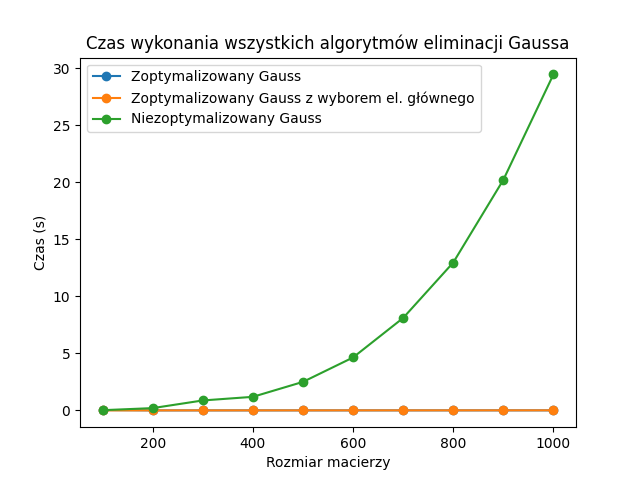
\includegraphics[width=0.70\textwidth]{allTimePlot.png}
\caption{Czas wykonania wszystkich wersji eliminacji Gaussa w sekundach na losowych macierzach wygenerowanych przez funkcję \texttt{matcond}.}
\end{figure}

\begin{figure}[H]
\centering
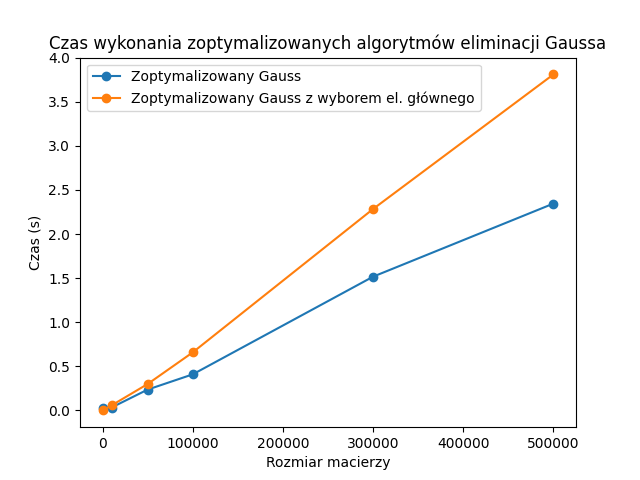
\includegraphics[width=0.70\textwidth]{timePlot.png}
\caption{Czas wykonania zoptymalizowanych wersji eliminacji Gaussa w sekundach na macierzach testowych.}
\end{figure}

\begin{figure}[H]
\centering
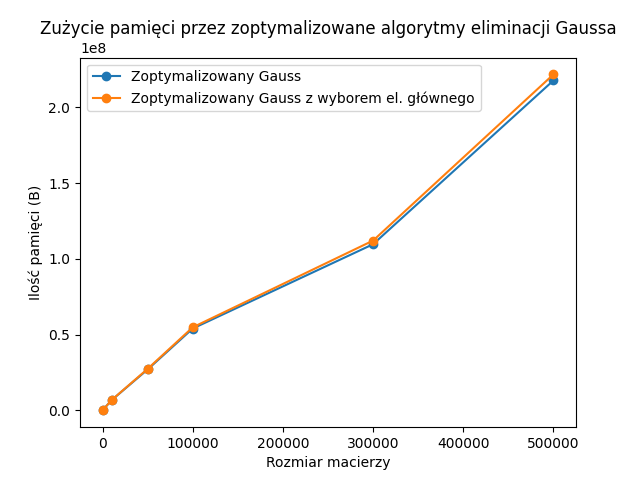
\includegraphics[width=0.70\textwidth]{memoryPlot.png}
\caption{Zużycie pamięci przez zoptymalizowane wersje eliminacji Gaussa w bajtach na macierzach testowych.}
\end{figure}

\subsection{Obserwacje i wnioski}
Tak jak się spodziewaliśmy, zoptymalizowane wersje elimiacji Gaussa działają znacznie szybciej od wersji niedostosowanej pod zadane macierze.
Faktycznie działają one w czasie liniowym.
Wersja bez wyboru elementu głównego jest szybsza, ale trzeba pamiętać o jej ograniczeniach w kontekście obliczeń numerycznych.
Na wykresach widać, że wersja z częściowym wyborem elementu głównego zużywa odrobinę więcej pamięci, jako że musi jeszcze przechować wektor permutacji.\\

Poczyniona w tym zadaniu optymalizacja była ogromna - złożoność została ograniczona z $O(n^3)$ do $O(n)$.
Co ciekawe, zoptymalizowana wersja eliminacji Gaussa była bardzo zbliżona do oryginalnej.
Wystraczyło ograniczyć liczbę elementów do wyzerowania, co świetnie wpłynęło na osiągi.\\

Wniosek z tego taki, że należy poświęcać czas na dokładną analizę problemu i tego z jakimi danymi pracujemy.
To zadanie dobrze pokazało, że czasami duże optymalizacje da się poczynić małym kosztem.

\end{document}
